\documentclass[a4paper,ngerman, headheight=28pt,12pt]{scrartcl}
  
  
% PACKAGES  
\usepackage[a4paper,left=3cm,right=4cm,top=2.5cm,bottom=2.5cm]{geometry}

\usepackage{fontspec}
\usepackage{babel}
\usepackage{csquotes}
\usepackage{relsize}
\usepackage{setspace}

\usepackage{lineno}

\usepackage{tabularray}
\usepackage{float}

% Title Spacing

\RedeclareSectionCommand[
  %runin=false,
  afterindent=false,
  beforeskip=.5\baselineskip,
  afterskip=.25\baselineskip]{section}
\RedeclareSectionCommand[
  %runin=false,
  afterindent=false,
  beforeskip=.25\baselineskip,
  afterskip=.125\baselineskip]{subsection}
\RedeclareSectionCommand[
  %runin=false,
  afterindent=false,
  beforeskip=.175\baselineskip,
  afterskip=.0625\baselineskip]{subsubsection}


% Literaturverzeichnis
\usepackage[
backend=biber,
style=alphabetic,
sorting=ynt,
maxbibnames=99
]{biblatex}

\addbibresource{refs_facharbeit.bib}

\DeclareLabelalphaTemplate{
  \labelelement{
    \field[final]{shorthand}
    \field{label}
    \field[strwidth=2,strside=left,ifnames=1]{labelname}
    \field[strwidth=1,strside=left]{labelname}
  }
  \labelelement{
    \field[strwidth=2,strside=right]{year}
  }
}

\setmainfont{Calibri}
\MakeOuterQuote{"}

\newcommand{\LongMinus}{–}


% Die nächsten vier Felder bitte anpassen:
\newcommand{\Titel}{Dezentralisierte asymmetrische \\ Verschlüsselung über Tor} % Titel für Facharbeit
\newcommand{\SubTitel}{Die Lösung für sicheres Messaging?}

\newcommand{\PageTitel}{Dezentralisierte asymmetrische Verschlüsselung \\ über Tor \LongMinus{} Die Lösung für sicheres Messaging?} % Seitentitel für Facharbeit
\newcommand{\Author}{Hendrik Lind}     % Ich
\newcommand{\Department}{Seminarfach Informatik}
\newcommand{\School}{Windthorst-Gymnasium Meppen}
\newcommand{\Country}{Deutschland}
\newcommand{\Abgabe}{20. November 2023}

\newcommand{\thesisDegree}{Facharbeit}
\newcommand{\faculty}{Seminarfach Informatik}
\newcommand{\thesisPlaceDate}{\today}

\newcommand{\vcite}[1]{\cite[vgl.][]{#1}}


% Kopf- und Fußzeilen
\usepackage{scrlayer-scrpage, lastpage}
\setkomafont{pageheadfoot}{\large\textrm}
\lohead{\PageTitel}
\rohead{\Author}
\cfoot*{\thepage{}/\pageref{LastPage}}

% Position des Titels
\usepackage{titling}
\setlength{\droptitle}{-1.0cm}


% Für mathematische Befehle und Symbole
\usepackage{amsmath}
\usepackage{amssymb}
\usepackage{wrapfig}

% Für Bilder
\usepackage{graphicx}
\usepackage{graphbox}

% Für Algorithmen
\usepackage{algpseudocode}

% Für Quelltext
\usepackage{listings}
\usepackage{color}


\graphicspath{ {./img/} }


% 1.5 Line spacing
\setstretch{1.5}


% Defining rust langauge
\definecolor{GrayCodeBlock}{RGB}{241,241,241}
\definecolor{BlackText}{RGB}{110,107,94}
\definecolor{RedTypename}{RGB}{182,86,17}
\definecolor{GreenString}{RGB}{96,172,57}
\definecolor{PurpleKeyword}{RGB}{184,84,212}
\definecolor{GrayComment}{RGB}{170,170,170}
\definecolor{GoldDocumentation}{RGB}{180,165,45}
\lstdefinelanguage{rust}
{
    columns=fullflexible,
    keepspaces=true,
    frame=single,
    framesep=0pt,
    framerule=0pt,
    framexleftmargin=4pt,
    framexrightmargin=4pt,
    framextopmargin=5pt,
    framexbottommargin=3pt,
    xleftmargin=4pt,
    xrightmargin=4pt,
    backgroundcolor=\color{GrayCodeBlock},
    basicstyle=\ttfamily\color{BlackText},
    keywords={
        true,false,
        unsafe,async,await,move,
        use,pub,crate,super,self,mod,
        struct,enum,fn,const,static,let,mut,ref,type,impl,dyn,trait,where,as,
        break,continue,if,else,while,for,loop,match,return,yield,in
    },
    keywordstyle=\color{PurpleKeyword},
    ndkeywords={
        bool,u8,u16,u32,u64,u128,i8,i16,i32,i64,i128,char,str,
        Self,Option,Some,None,Result,Ok,Err,String,Box,Vec,Rc,Arc,Cell,RefCell,HashMap,BTreeMap,
        macro_rules
    },
    ndkeywordstyle=\color{RedTypename},
    comment=[l][\color{GrayComment}\slshape]{//},
    morecomment=[s][\color{GrayComment}\slshape]{/*}{*/},
    morecomment=[l][\color{GoldDocumentation}\slshape]{///},
    morecomment=[s][\color{GoldDocumentation}\slshape]{/*!}{*/},
    morecomment=[l][\color{GoldDocumentation}\slshape]{//!},
    morecomment=[s][\color{RedTypename}]{\#![}{]},
    morecomment=[s][\color{RedTypename}]{\#[}{]},
    stringstyle=\color{GreenString},
    string=[b]"
}
% end

% Umlaute erlauben
\lstset{literate=%
  {Ö}{{\"O}}1
  {Ä}{{\"A}}1
  {Ü}{{\"U}}1
  {ß}{{\ss}}1
  {ü}{{\"u}}1
  {ä}{{\"a}}1
  {ö}{{\"o}}1
}
%end


\definecolor{mygreen}{rgb}{0,0.6,0}
\definecolor{mygray}{rgb}{0.5,0.5,0.5}
\definecolor{mymauve}{rgb}{0.58,0,0.82}
\lstset{
  keywordstyle=\color{blue},commentstyle=\color{mygreen},
  stringstyle=\color{mymauve},rulecolor=\color{black},
  basicstyle=\footnotesize\ttfamily,numberstyle=\tiny\color{mygray},
  captionpos=b, % sets the caption-position to bottom
  keepspaces=true, % keeps spaces in text
  numbers=left, numbersep=5pt, showspaces=false,showstringspaces=true,
  showtabs=false, stepnumber=2, tabsize=2, title=\lstname{}
}
\lstset{language=Rust}          % Set your language (you can change the language for each code-block optionally)

% Diese beiden Pakete müssen zuletzt geladen werden
\usepackage[hidelinks]{hyperref} % Anklickbare Links im Dokument
\usepackage{cleveref}


% Titlepage required things


% Necessary packages for the titlepage:
\usepackage{tikz}
\usetikzlibrary{calc}
%\usepackage{graphicx}
% \usepackage{newtxtext}
%\usepackage{float}
\usepackage{comment}
% This command changes the font style where SLU promotes Arial
%\newenvironment{myfont}{\fontfamily{phv}\selectfont}{\par}




% Facharbeit

\begin{document}
% To add this template to the main.tex file, just add the command "% To add this template to the main.tex file, just add the command "% To add this template to the main.tex file, just add the command "\include{titlePageSLU} after "\begin{docuemnt}" in the main.tex file


% In this segment, enter the desired data to be shown at the title page
\newcommand{\thesisAuthor}{Firstname Lastname}
\newcommand{\thesisTitle}{Interesting Thesis Title}
\newcommand{\thesisSubTitle}{little bit more descriptive}
\newcommand{\thesisTitleTranslated}{Translated Headline}
\newcommand{\thesisDegree}{Master thesis project}
\newcommand{\university}{Swedish University of Argicultural Science, SLU}
\newcommand{\credits}{30 hp}
\newcommand{\faculty}{Faculty of blablabalba}
\newcommand{\thesisPlaceDate}{Place of puplication, Year}
\newcommand{\company}{Company name}

%------------------------------------------------------------------------------
\begin{titlepage}
\thispagestyle{empty}
\myfont

% Use this line of code if both SLU loggo and company/other institution loggo is desired. The positions are possible to change with the \hspace and \vspace syntax.
\begin{figure} [H]
\vspace{-3cm}
 \centering
\begin{minipage}[t]{.45\linewidth}
  \raggedright
  % Upload and include SLU loggo here:
  \hspace*{-2cm}
\includegraphics[width=\linewidth]{slu_logo_webb.png}
  
\end{minipage}%
  \begin{minipage}[t]{.45\linewidth}
  \vspace{-3.3cm}
 \raggedleft
% Upload and include other loggo here (loggo of wikipedia is used as an example):
 \hspace*{1cm}
\includegraphics[width =0.5\textwidth]{wikilogo.png} \hspace*{-1cm}
 
\end{minipage}
\end{figure}


% If only the logo for SLU is desired, delete "\begin{comment}" and "\end{comment}" to use this line of code:
\begin{comment}
\begin{figure}
\vspace{-3cm}
    \hspace*{-2cm}
\includegraphics[width = 0.3\textwidth]{slu_logo_webb.png}\hspace*{-2cm}
\end{figure}
\end{comment}


% Adds background picture. Delete code if no background picture is wanted.
\begin{tikzpicture}[overlay, remember picture]
\node[anchor=south west, 
      xshift=-0.2cm, 
      yshift=-0.2cm] 
     at (current page.south west)
     {
\includegraphics[width = 1.8\textwidth, height = 9cm]{background.png}}; 
\end{tikzpicture}


\vspace{1cm}
\par
\noindent
\Huge
\textbf{\thesisTitle}
\vspace{0.2cm}
\LARGE
\par
\noindent
- \thesisSubTitle\\
\rule[0.3cm]{\linewidth}{2pt}
\Large

% Delete this line if no translation is desired
\noindent
\textit{\thesisTitleTranslated}

\vspace{2cm}
\noindent
\LARGE
\thesisAuthor\\
\vspace{4 cm}
\small
\par \noindent
\thesisDegree $\cdot$ \credits
\par \noindent
\university
\par \noindent
\faculty
\par \noindent
\company
\par \noindent
\thesisPlaceDate

\end{titlepage}
 after "\begin{docuemnt}" in the main.tex file


% In this segment, enter the desired data to be shown at the title page
\newcommand{\thesisAuthor}{Firstname Lastname}
\newcommand{\thesisTitle}{Interesting Thesis Title}
\newcommand{\thesisSubTitle}{little bit more descriptive}
\newcommand{\thesisTitleTranslated}{Translated Headline}
\newcommand{\thesisDegree}{Master thesis project}
\newcommand{\university}{Swedish University of Argicultural Science, SLU}
\newcommand{\credits}{30 hp}
\newcommand{\faculty}{Faculty of blablabalba}
\newcommand{\thesisPlaceDate}{Place of puplication, Year}
\newcommand{\company}{Company name}

%------------------------------------------------------------------------------
\begin{titlepage}
\thispagestyle{empty}
\myfont

% Use this line of code if both SLU loggo and company/other institution loggo is desired. The positions are possible to change with the \hspace and \vspace syntax.
\begin{figure} [H]
\vspace{-3cm}
 \centering
\begin{minipage}[t]{.45\linewidth}
  \raggedright
  % Upload and include SLU loggo here:
  \hspace*{-2cm}
\includegraphics[width=\linewidth]{slu_logo_webb.png}
  
\end{minipage}%
  \begin{minipage}[t]{.45\linewidth}
  \vspace{-3.3cm}
 \raggedleft
% Upload and include other loggo here (loggo of wikipedia is used as an example):
 \hspace*{1cm}
\includegraphics[width =0.5\textwidth]{wikilogo.png} \hspace*{-1cm}
 
\end{minipage}
\end{figure}


% If only the logo for SLU is desired, delete "\begin{comment}" and "\end{comment}" to use this line of code:
\begin{comment}
\begin{figure}
\vspace{-3cm}
    \hspace*{-2cm}
\includegraphics[width = 0.3\textwidth]{slu_logo_webb.png}\hspace*{-2cm}
\end{figure}
\end{comment}


% Adds background picture. Delete code if no background picture is wanted.
\begin{tikzpicture}[overlay, remember picture]
\node[anchor=south west, 
      xshift=-0.2cm, 
      yshift=-0.2cm] 
     at (current page.south west)
     {
\includegraphics[width = 1.8\textwidth, height = 9cm]{background.png}}; 
\end{tikzpicture}


\vspace{1cm}
\par
\noindent
\Huge
\textbf{\thesisTitle}
\vspace{0.2cm}
\LARGE
\par
\noindent
- \thesisSubTitle\\
\rule[0.3cm]{\linewidth}{2pt}
\Large

% Delete this line if no translation is desired
\noindent
\textit{\thesisTitleTranslated}

\vspace{2cm}
\noindent
\LARGE
\thesisAuthor\\
\vspace{4 cm}
\small
\par \noindent
\thesisDegree $\cdot$ \credits
\par \noindent
\university
\par \noindent
\faculty
\par \noindent
\company
\par \noindent
\thesisPlaceDate

\end{titlepage}
 after "\begin{docuemnt}" in the main.tex file


%------------------------------------------------------------------------------
\begin{titlepage}
\thispagestyle{empty}
% Use this line of code if both SLU loggo and company/other institution loggo is desired. The positions are possible to change with the \hspace and \vspace syntax.
\begin{figure} [H]
\vspace{-2cm}
 \centering
\begin{minipage}[t]{.45\linewidth}
  \raggedright
  % Upload and include SLU loggo here:
  \hspace*{-2cm}
\includegraphics[width=\linewidth]{wgm.png}
  
\end{minipage}%
  \begin{minipage}[t]{.45\linewidth}
  \vspace{-3.3cm}
 \raggedleft
% Upload and include other loggo here (loggo of wikipedia is used as an example):
 \hspace*{2cm}
\includegraphics[width =0.5\textwidth]{enkrypton.png} \hspace*{-1cm}
 
\end{minipage}
\end{figure}

% Adds background picture. Delete code if no background picture is wanted.
\begin{tikzpicture}[overlay, remember picture]
\node[anchor=south west, 
      xshift=-0.2cm, 
      yshift=-0.2cm] 
     at (current page.south west)
     {
\includegraphics[width = 1.8\textwidth, height = 9cm]{background.png}}; 
\end{tikzpicture}


\vspace{1cm}
\par
\noindent
\Huge
\textbf{\Titel}
\vspace{0.2cm}
\LARGE
\par
\noindent
\SubTitel\\
\rule[0.3cm]{\linewidth}{2pt}
\Large

\vspace{2cm}
\noindent
\LARGE
\Author\\
\vspace{4 cm}
\small
\par \noindent
\thesisDegree
\par \noindent
\School
\par \noindent
\faculty
\par \noindent
\thesisPlaceDate

\end{titlepage}
\tableofcontents
\setcounter{page}{0}
\thispagestyle{empty}
\vspace{0.5cm}
\pagebreak


\linenumbers{}
\modulolinenumbers[5]
\section{Einleitung}
%//SECTION Einleitung
Russland, China, Iran. In all diesen totalitären Staaten herrscht eine starke Zensur \vcite{AmnReport}. % check for Russia and North Korea as well
Rund 1,7 Milliarden Menschen sind allein nur in diesen drei Staaten von der Einschränkung der Meinungsfreiheit betroffen \vcite{UnPop}. Wie können Bürger
dieser Staaten ihre Meinung also verbreiten und andere Staaten auf
%//TODO hier staatskritisch ist falsches wort mir fällt aber das richtige nicht ein
staatskritische Probleme aufmerksam machen ohne sich selber in Gefahr zu bringen?
%//!SECTION
%//SECTION Problemstellung
\\
%//TODO Hier nochmal nach einer anderen Quelle suchen, die passt nicht 100%ig
Bei herkömmlichen Messengern, wie Whatsapp, Signal und co., braucht die Außenwelt die Telefonnummern der im totalitären Staat wohnenden Bürgern und Reportern, um diese zu kontaktieren. Allerdings könnte ein totalitärer Staat, sich als Empfänger ausgeben, sodass Bürger/Reporter ihre private Nummer an den Staat überreichen und dieser somit jene Nummer rückverfolgen kann \vcite{LocPolice}.
Und genau hier liegt das Problem: Bürger und Reporter können nicht durch alltägliche Messenger mit der Außenwelt kommunizieren, da der Staat deren Nummer zurückverfolgen kann und somit weiter die Meinungsfreiheit einschränkt und unterbindet.
\\
Durch die zentrale Infrastruktur, welche die meisten Messenger, wie zum Beispiel WhatsApp und Signal verwenden, ist es für totalitäre Staaten, wie China, möglich, die IP-Adressen jener Server zu blockieren und somit für Bürger und Reporter unzugänglich zu machen \vcite{ChinaFirewall}.
\\
%//!SECTION
%//SECTION Lösungsvorschlag / Ziel
Ein dezentralisierter Messenger, welcher Ende-zu-Ende verschlüsselt ist und über das Tor-Netzwerk kommuniziert, könnte bei diesen Problemen eine Lösung sein. Die Frage, ob ein solcher Messenger die Lösung für Bürger eines totalitären Staates ist, soll in dieser Arbeit geklärt werden.
%//!SECTION
\\
%//SECTION Kapitel
%//TODO besser die Kapitel und so beschreiben, ist bis jetzt quatsch
%//REVIEW - Wirklich nur asymmetrische Verschlüsselung?
Um diese Frage beantworten zu können, beschäftigt sich diese Arbeit in dem zweiten Kapitel mit der asymmetrischen Verschlüsselung, welche benötigt wird um die Ende-zu-Ende-Verschlüsselung (E2EE) umzusetzen und die Definition der E2EE und asymmetrischen Verschlüsselung \vcite{E2EE-Method}.
Das dritte Kapitel beinhaltet eine mögliche Lösung, um eine Anonymität über das Internet zu gewährleisten, wobei das Tor-Netzwerk eine wichtige Rolle spielt.
Im vierte Kapitel befasst sich diese Arbeit mit einer Dezentralisierung der Infrastruktur, um eine weitere Sicherheitsebene zu schaffen.
Zuletzt werden im fünften Kapitel die Vor- und Nachteile eines solchen Messengers betrachtet, im sechsten Kapitel wird eine mögliche Umsetzung des Messengers beschrieben und im siebten Kapitel wird ein Fazit gezogen.
%//!SECTION



\section{Asymmetrische Verschlüsselung}
%//SECTION E2EE und asymmetrische Verschlüsselung
Um einen sicheren Nachrichtenaustausch zu gewährleisten, wird in dieser Arbeit die E2EE implementiert. Bei der E2EE wird von dem Sender die Nachricht, bevor sie an den Empfänger geschickt wird, verschlüsselt \vcite{E2EE}. Dazwischenliegende Akteure, wie zum Beispiel Server oder mögliche Angreifer, können demzufolge die Nachricht nicht lesen. \textbf{Nur} der Empfänger der Nachricht kann diese auch entschlüsseln. Als Ent- und Verschlüsselungsverfahren der Nachrichten wird die asymmetrische Verschlüsselung verwendet.
%//REVIEW - RSA-Verfahren überprüfen bzw. jetzt schon erwähnen? und okay dass ich sage gängigste Verfahren?
Für diese Arbeit werde ich die gängigste asymmetrische Verschlüsselung, das RSA-Verfahren, verwenden.
%//!SECTION
\subsection{Grundlagen}
%//SECTION Grundlagen
%//REVIEW - Kann ich hier auch einfach nur einmal zitieren? Eigentlich ist in der Literatur alles gleich hierzu oder muss ich jedes mal ne neue Quelle für jeden Satz finden?
Grundsätzlich gibt es bei der asymmetrischen Verschlüsselung ein Schlüsselpaar (Keypair), welches aus einem privaten Schlüssel (private key) und einem öffentlichen Schlüssel (public key) besteht \vcite{Rsa-Basics}. Diese beiden Schlüssel hängen mathematisch zusammen, sodass der öffentliche Schlüssel Nachrichten \textbf{nur} verschlüsseln und nicht entschlüsseln kann. \textbf{Nur} der zum Schlüsselpaar dazugehörige private Schlüssel ist in der Lage, die verschlüsselte Nachricht wieder zu entschlüsseln (siehe \cref{fig:E2EE}).

%//REVIEW - Wie Anhang mit Bildern und so?
\begin{figure}[h]
  \centering
  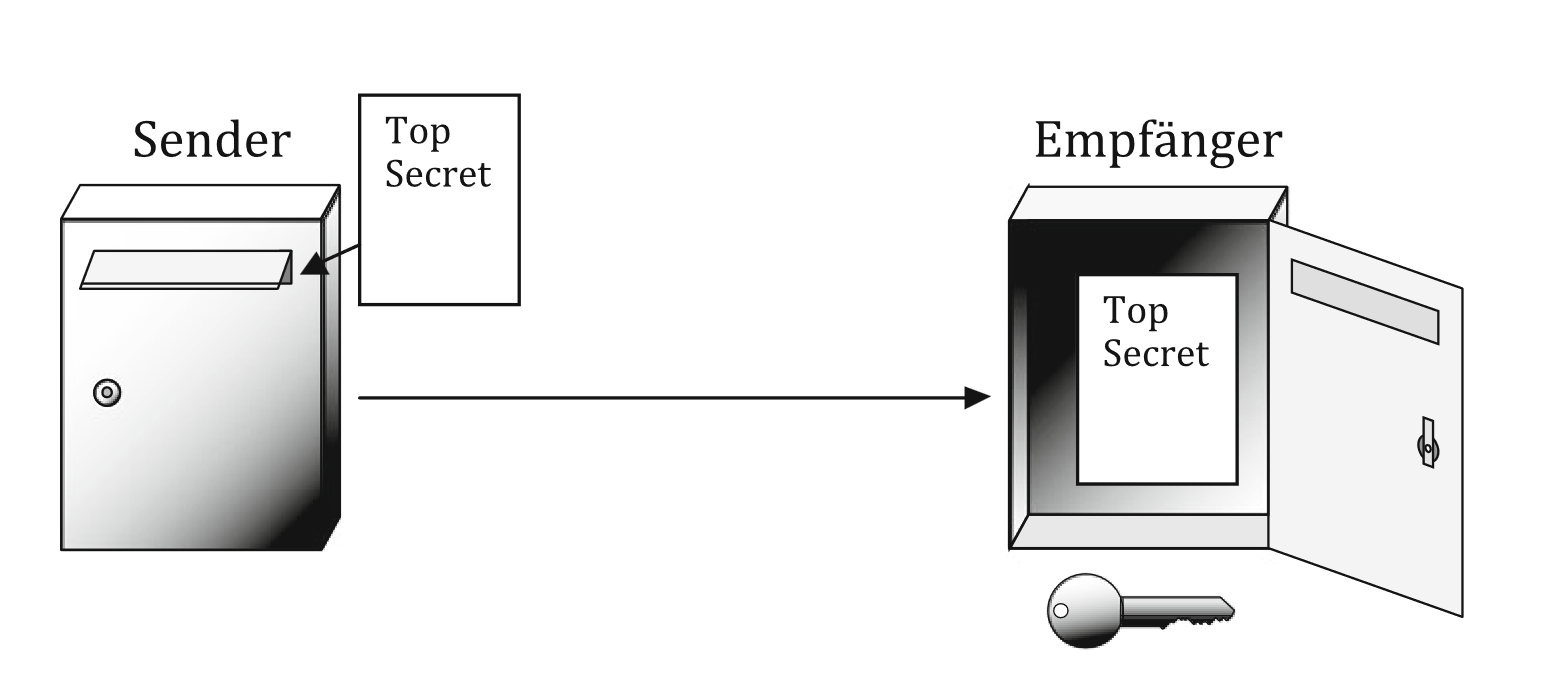
\includegraphics[width=0.75\textwidth]{Briefkasten-asymm.png}
  \caption{Jeder Sender kann mit dem öffentlichen Schlüssel die Nachricht "verschlüsseln" (also in den Briefkasten eine Nachricht werfen), aber nur der Empfänger kann den Briefkasten mit seinem privaten Schlüssel öffnen \vcite{fig:Rsa-Cryptography} \label{fig:E2EE}}
\end{figure}
%//!SECTION

%//TODO insgesamt noch mehr Quellen finden, habe die ganze Rechnung aus 1 bis 2 Quellen
\subsection{Mathematische Betrachtung}
Alle Variablen der folgenden Berechnungen liegen im Bereich $\mathbb{N}$. \\
Für die Generierung des Schlüsselpaares benötigen wir zuerst zwei große zufällige Primzahlen, $P$ und $Q$. Daraus ergibt sich $n = P * Q$, wobei $P \neq Q$, sodass $P$ bzw. $Q$ nicht durch $\sqrt{n}$ ermittelt werden kann \vcite{RsaGenCond}. Der private Schlüssel besteht aus den Komponenten $\{ n, d \}$ währenddessen der öffentliche Schlüssel aus $\{ n, e \}$ besteht \vcite{RsaVariables}.
\subsubsection{Eulersche Phi-Funktion}
Die Eulersche Phi-Funktion spielt eine wichtige Rolle in dem RSA-Verfahren \vcite{TotientFuncMultiplicative}. Grundsätzlich gibt $\phi(x)$ an, wie viele positive teilerfremde Zahlen bis $x$ existieren (wo also der größte gemeinsamer Teiler ($\gcd$) $1$ ist) \vcite{EulersTotientFunction}. Somit ergibt $\phi(6) = 2$  oder bei einer Primzahl $\phi(7) = 7 - 1 = 6$ somit $\phi(x) = x-1$, wenn $x$ eine Primzahl ist, da jede Zahl kleiner als $x$ teilerfremd sein muss.
%//REVIEW - Nachfragen ob ich auch noch \prod und die Gleichung an sich erklären muss
%//TODO - Gleichung und Stuff erklären
\begin{equation*}
  \begin{aligned}
    \phi(n) & = \phi(P \cdot Q)                                                \\
    \phi(n) & = \phi(P) \cdot \phi(Q)                                          \\
    \phi(P) & = P -1                                          & \phi(Q) = Q -1 \\
    \phi(n) & = \left(P - 1 \right) \cdot \left( Q - 1\right)
  \end{aligned}
\end{equation*}
%//REVIEW - Wie zitieren von mathematischem Kram?
\vcite{TotientFuncMultiplicative}
\subsubsection{Generierung des Schlüsselpaares}
Sowohl der private als auch der öffentliche Schlüssel besteht unter anderem aus folgender Komponente: $n = P \cdot Q$.
Für den öffentlichen Schlüssel benötigen wir die Komponente $e$, welche zur Verschlüsselung einer Nachricht benötigt wird. $e$ ist hierbei eine zufällige Zahl, bei welcher folgende Bedingungen gelten \vcite{RsaMaths1}:
\begin{equation*}
  e = \begin{cases}
    1 < e < \phi(n)  \\
    \gcd(e, \phi(n)) = 1 \\
    \text{$e$ kein Teiler von $\phi(n)$}
  \end{cases}
\end{equation*}
Mit der errechneten Komponente $e$, welche Nachrichten verschlüsselt, kann der öffentliche Schlüssel nun an den Sender übermittelt werden.

Um den privaten Schlüssel zu berechnen benötigen wir die Komponente $d$, welche zur Entschlüsselung verwendet wird \vcite{RsaEncryptionDecryption}.
%//REVIEW - explain what mod is as well?
\begin{equation*}
  \begin{aligned}
    \phi(n) & = (P-1)(Q-1)     \\
    e * d   & = 1 \mod \phi(n)
  \end{aligned}
\end{equation*}
%//REVIEW - Wie zitiere ich hier und nen vernünftiges Ende hierfür finden

\subsection{Sicherheit}
%//NOTE - Maybe brauche ich das noch aber eig nicht oder?
%\subsection{Vergleich zur symmetrischen Verschlüsselung}
Das RSA-Verfahren macht sich die Trapdoor-Einwegfunktion zu Nutze. Das bedeutet, dass eine Funktion mit modernen Computern unmöglich ist, zu invertieren, wenn eine Komponente fehlt (in diesem Fall $d$). Wenn diese jedoch gegeben ist, ist die Umkehroperation leicht. Zu sehen ist dies bei der Ver-/Entschlüsselung von Nachrichten mit dem öffentlichen und privaten Schlüssel \vcite{RsaTrapdoor}.
\begin{equation*}
  \begin{aligned}
    c &= m^e \mod n & \text{Verschlüsselung zu $c$ mit $m$ als Nachricht} \\
    m &= c^d \mod n & \text{Umkehroperation (Entschlüsslung) von $c$ zu $m$}
  \end{aligned}
\end{equation*}
Um die verschlüsselte Nachricht $c$ zu entschlüsseln, bräuchte ein möglicher Angreifer die Komponente des privaten Schlüssels $d$. Diese ist allerdings schwer zu berechnen, da, wie schon vorher bereits gezeigt, dafür $\phi(n)$ benötigt wird. Auch $\phi(n)$ ist rechenaufwendig, da dafür eine Primfaktorzerlegung von $n$ benötigt wird. Wichtig hierbei ist aber, dass die Länge von $n$ (Schlüssellänge) mindestens 3000 Bit betragen sollte, da sonst die Primfaktorzerlegung von $n$ mit modernen Computern möglich sein könnte \vcite{RsaKeyLength}.
%//REVIEW - Zitierweise hier richtig? Weil is so von BSI und so


\section{Anonymität mit dem Tor-Netzwerk}
\subsection{Sicherheit}


\section{Dezentralisierung}
\subsection{Sicherheit}


\section{Vor- und Nachteile}
\subsection{Kriminalität}
\subsection{freie Meinungsäußerung}

\section{programmatische Umsetzung}

\section{Fazit}

\pagebreak
\nolinenumbers{}
\printbibliography[notkeyword={figure}]
\printbibliography[heading=subbibliography,title={Anhang},keyword={figure}]

\end{document}
